\section{Hashmaps}%
\label{sec:hashmaps}

\begin{frame}
	\frametitle{Hashmaps}
	\framesubtitle{Have fun figuring out what this map represents.}
	\begin{center}
		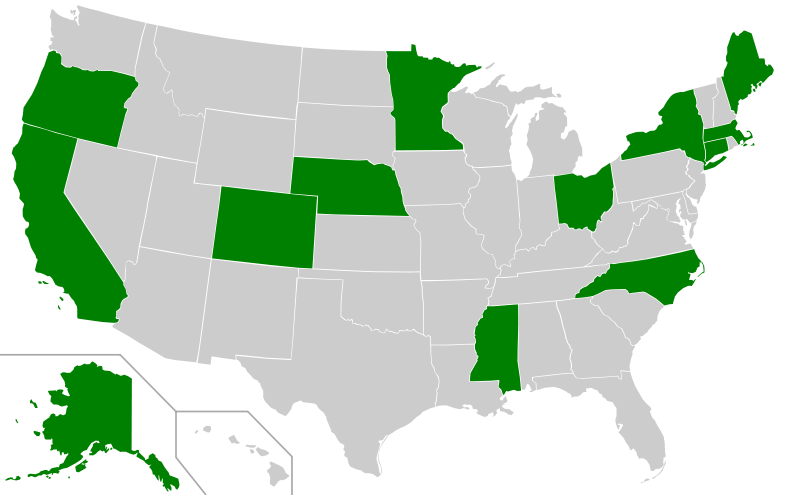
\includegraphics[width=0.6\textwidth]{figures/hashmap.png}\\
		\hspace*{15pt}\hbox{\scriptsize Image By:\thinspace{\itshape Photohound}}
	\end{center}
\end{frame}

\begin{frame}
	\frametitle{Hashmaps}
		\begin{block}{Hashmaps}
			Implement the Map ADT using Hash tables.\\
			\pause
			With a good hash function, we expect: $\Theta(1)$ insertion/deletion/retrieval.\\
			But worst-case they are still $\Theta(n)$.
		\end{block}	
		\pause
		\begin{problemblock}{Handling hashing conflicts}
			Different options to handle hash conflicts:
			\begin{itemize}
				\item Separate Chaining
				\item (Linear) Probing
			\end{itemize}
		\end{problemblock}
\end{frame}

\begin{frame}
	\frametitle{Lets start with the basics}
	\vspace{-13pt}
	\begin{columns}
		\column{0.355\textwidth}
		\begin{itemize}
			\item Creating a new hashmap
			\item<2-> Getting the size
			\item<3-> A hash function for keys in this map
			\item<4-> Getting an item
			\item<4-> Putting an item
		\end{itemize}
		\column{0.555\textwidth}
			
		\lstinputlisting[basicstyle=\tiny\ttfamily,linebackgroundcolor={%
			\btLstHL<1>{3-5}%
			\btLstHL<2>{7-8}%
			\btLstHL<3>{10-11}%
			\btLstHL<4>{13-15}%
			\btLstHL<5>{17-21}%
		}]
		{code/hashmap.py}
	\end{columns}
	\only<5->{
			\begin{block}{So conclusion}
				It depends on how we put things into the buckets!\\
				Do we use the linked list? Or do we do something else?
			\end{block}	
	}
\end{frame}
